%!TEX root=../main.tex
\chapter{Projektmanagement}
Aufgrund der zeitlichen Befristung und der erheblichen Komplexität von \textit{Refundable} ist es von Nöten, eine passende Projektmanagementmethode zu wählen. Zuerst gilt es aber zu klären, was der Begrigg Projektmanagement (\Gls{pm}) überpaupt bedeutet.\\
\begin{center}
	\textit{\enquote{Das \Gls{pm} umfasst die Führungsaufgaben, -organisation, -techniken und -mittel zur erfolgreichen Abwicklung eines Projekts. Die \Gls{din} 69901 definiert Projektmanagement als Gesamtheit von Führungsaufgaben, -organisation, -techniken und -mittel für die Abwicklung eines Projekts. Allgemeiner definiert das Project Management Institute (\Gls{pmi}) im \Gls{pmbok} \Gls{pm} als Anwendung von Wissen, Fähigkeiten, Methoden und Techniken auf die Vorgänge innerhalb eines Projekts}}\cite{pm-definition}.
\end{center}
Da das Projektteam hat während seiner Zeit am TGM im Rahmen des \Gls{itp} Unterrichts vor allem mit der traditionellen Methode, dem Wasserfallmodell und den zwei agilen Methoden, Scrum und Kanban gearbeitet und sich mit diesen Methoden am Besten auskennt, wird sich in \autoref{chapter:tradi-pm} und \autoref{chapter:agil-pm} auf diese Methoden beschränkt.
\newpage
\section{Traditionelles Projektmanagement}
\label{chapter:tradi-pm}
Das traditionelle Projektmanagement hat einen linearen Ablauf. Das heißt, man notiert sich alle Aufgaben, die man abzuarbeiten Hat und arbeitet sie alle der Reihe nach ab. Keine neue Aufgabe wird angefangen, bis diejenige davor abgearbeitet ist. Ein sehr wichtiger Punkt in diesem Managementsystem ist die viele Dokumentation, ohne diese funtkioniert das System nicht. Verkörpert wird dieses Verfahren durch das Wasserfallmodell:
\begin{figure}[H]
	\centering
	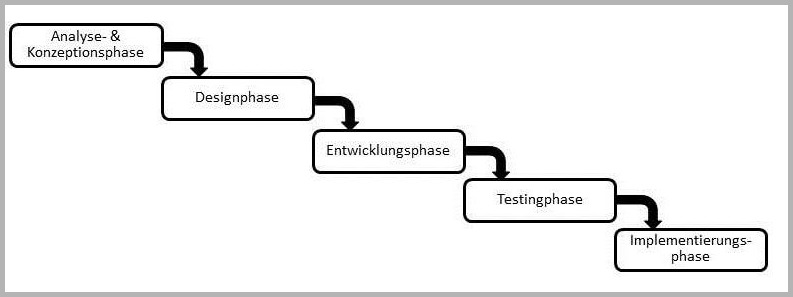
\includegraphics[width=0.7\linewidth]{images/projektmanagement/wasserfallmodell}
	\caption[Wasserfallmodell]{Illustration des Wasserfallmodells \cite{pm-wasserfall-online}}
	\label{fig:wasserfall}
\end{figure}
\subsection{Analyse und Konzeptionsphase}
In dieser Phase wird die Machbarkeit (Kosten, Ertrag, Realisierbarkeit, etc.) des Projektes mittels einer Machbarkeitsstudie analysiert \cite{pm-wasserfall-ionos}. Danach wird ein Lastenheft und ein Projektstrukturplan erstellt. In der Anforderungsdefinition, werden alle möglichen Funktionen definiert, die das Software-Projekt beinhalten soll und kann. Diese werden im Pflichtenheft notiert. Alljene Dinge, die in der Analysephase nicht bedacht werden, können im Laufe des Projektes gravierende Folgen auslösen \cite{pm-wasserfall-online}.
\subsection{Designphase}
Die Designphase wird streng in Kundenkontakt durchgeführt \cite{pm-wasserfall-online} und ist dafür da, dass ein konkreter Lösungsvorschlaf, mit den definierten Anforderungen ausgearbeitet wird \cite{pm-wasserfall-ionos}. Es wird eine detaillierte Anleitung für die Erstellung der Software verfasst, die sich vor allem auf Komponenten wie Schnittstellen, Frameworks oder Bibliotheken bezieht. Als Resultat dieser Phase erhält man ein Entwurfsdokument mit Software-Bauplan, als auch Testplänen, die sich auf einzelne Komponenten beziehen.
\subsection{Entwicklungsphase}
In dieser Phasae, werden die in der Designphase entwickelten Pläne umgesetzt. Der Projektleiter spielt hier eine tragende Rolle, denn er muss sich um externe, als auch interne Probleme kümmern und in Kontakt mit dem Auftraggeber bleiben \cite{pm-wasserfall-online}. 
\subsection{Testingphase}

\subsection{Implementierungsphase}
\section{Agiles Projektmanagement}
\label{chapter:agil-pm}
\subsection{Scrum}
\subsection{Kanban}
\section{Fazit}